\section{Funzionamento ad alto livello dei modelli di AI per Object Detection}

I modelli di intelligenza artificiale di Object Detection sono progettati per
identificare e localizzare oggetti specifici all'interno di immagini o video. 
Questa classe di modelli combina tecniche di computer vision e deep learning per
analizzare il contenuto visivo e riconoscere pattern associati a diverse categorie
di oggetti.

Il processo di  \textit{Object Detection} generalmente consiste in due fasi:
\begin{itemize}
    \item \textbf{Rilevamento delle regioni di interesse (Region Proposal):} In questa fase, il modello identifica le aree dell'immagine che potrebbero contenere oggetti. Tecniche come Selective Search o Region Proposal Networks (RPN) sono comunemente utilizzate per generare queste proposte.
    
    \item \textbf{Classificazione e localizzazione:} Una volta identificate le aree di interesse, il modello classifica ciascuna regione in una delle categorie predefinite e determina la posizione esatta dell'oggetto all'interno della regione tramite le \textbf{bounding box}.
\end{itemize}


\subsection{Le Bounding Box}

Come accennato in precedenza, le boundig box sono dei rettangoli che vengono 
utilizzati per localizzare gli oggetti all'interno di un' immaagine, o di un frame
nel caso di un video.
Esse sono definite da quattro coordinate: (x\textsubscript{min}, y\textsubscript{min})
e (x\textsubscript{max}, y\textsubscript{max}), che rappresentano gli angoli superiore
sinistro e inferiore destro del rettangolo, rispettivamente. Ad ogni bounding box
viene associata anche una \textbf{classe} che identifica il tipo di oggetto
rappresentato (ad esempio, persona, auto, cane, ecc.) e una \textbf{confidenza}
che indica la probabilità che l'oggetto rilevato appartenga a quella classe.

\begin{figure}[H]
    \centering
    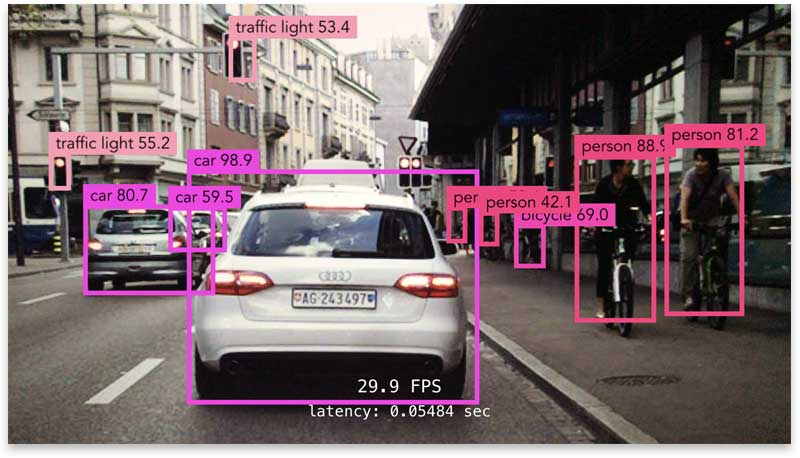
\includegraphics[width=0.5\textwidth]{images/car-bounding-boxes-sample.jpg}
        \caption{Un frame di una video camera, che mostra le vetture e semafori identificati da 
        bounding box, alle quali sono associati la classe e la confidenza.\\
        Fonte: \url{https://machinethink.net/blog/object-detection/}}
    \label{fig:bounding_box}
\end{figure}

Tuttavia, per motivi di semplicità e standardizzazione, le bounding box sono
solitamente definite all'interno di un file di annotazione associato all'immagine.
La struttura tipica di un dataset per l'addestramento e il test di modelli di Object Detection
viene rappresentato nel seguente modo:

\begin{figure}[H]
    \centering
    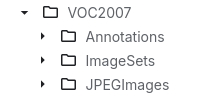
\includegraphics[width=0.5\textwidth]{images/OD-dataset-sample-pascal-voc-07.png}
        \caption{Esempio struttura tipica di un dataset per l'addestramento e il test di modelli di Object Detection, attraverso PASCAL VOC 2007.\\
        Fonte: \url{https://www.kaggle.com/datasets/zaraks/pascal-voc-2007}}
    \label{fig:dataset_structure}

\end{figure}

Una nota che vale la pena sottolineare ora ma che verrà approfondita più in avanti, è che il dataset non viene dato in pasto al modello
così com'è, perchè ogni modello, a seconda della sua architettura, richiede che i dati
siano formattati in un certo modo. Per questo motivo, prima di essere utilizzato per
l'addestramento, il dataset deve essere \textbf{preprocessato} per adattarsi ai requisiti specifici del modello scelto.


\subsection{L'importanza del dataset}
Il dataset in un contesto di Object Detection è un aspetto cruciale per il successo
dell'addestramento di un modello focalizzato su questo specifico compito.
Il dataset non deve avere solo una quantità sufficente di immagini per ogni classe,
ma deve essere anche il più vario e ampio possibile, permettendo al modello di
imparare a riconoscere gli oggetti in diverse condizioni.
Infatti il riconoscimento di oggetti viene influenzato da molteplici fattori, tra cui:

\begin{itemize}
    \item \textbf{Angolazione e prospettiva:} Una delle difficoltà 
    principali nell'addestramento di modelli di Object Detection è la variazione
    della prospettiva da cui un oggeetto può essere visto. Variando l'Angolazione
    cilindro può apparire come un cerchio, un ovale o un rettangolo, a seconda
    dell'angolazione da cui viene osservato.

    \item \textbf{Illuminazione e condizioni ambientali:} L'illuminazione ha una grande
    influenza sulla definizione e visibilità degli oggetti. Anche in questo caso,
    un oggetto può apparire molto diverso in condizioni di luce intensa rispetto
    a condizioni di scarsa illuminazione. Inoltre, condizioni atmosferiche come
    pioggia, nebbia o neve possono ulteriormente complicare il riconoscimento
    degli oggetti.

    \item \textbf{Occlusione:} Gli oggetti possono risultare parzialmente nascosti da altri oggetti
    o elementi nell'ambiente. Questo fenomeno,  rappresenta una  sfida significativa
    per i modelli di Object Detection, poichè devono essere in grado di identificare
    gli oggetti anche quando non sono completamente visibili.

\end{itemize}

Il dataset è quindi un tassello fondamentale per l'addestramento di questi modelli,
siccome quello che si vuole fare, è insegnare al modello a ottenere informazioni dalle
immagini, in modo che possa generalizzare e riconoscere gli oggetti in nuove immagini
mai viste prima.\\

La fase di addestramento la si analizzerà più avanti, durante la fase implementativa del progetto,
ma è importante sottolineare che il dataset viene solitamente pensato per essere suddiviso in tre sottoinsiemi distinti:
\begin{itemize}
    \item \textbf{Training set:} Utilizzato per addestrare il modello
    \item   \textbf{Validation set:} Utilizzato per ottimizzare i parametri del modello
    \item \textbf{Test set:} Utilizzato per valutare le prestazioni finali del modello
\end{itemize}

\subsection{Modello Faster R-CNN}


